
\section{Timing Measurements} 
\label{sec:timing} 

We characterize the timing performance of the CdTe sensor by measuring the timestamps
relative to the MCP-PMT device used as a reference timer. In 
Figure~\ref{fig:DeltaTVsAmplitude}, we show the dependence of the timestamp measurement 
on the amplitude of the signal, and observe no significant amplitude dependence.



%Fig: DeltaT vs Amplitude
\begin{figure}[htbp] 
\centering
%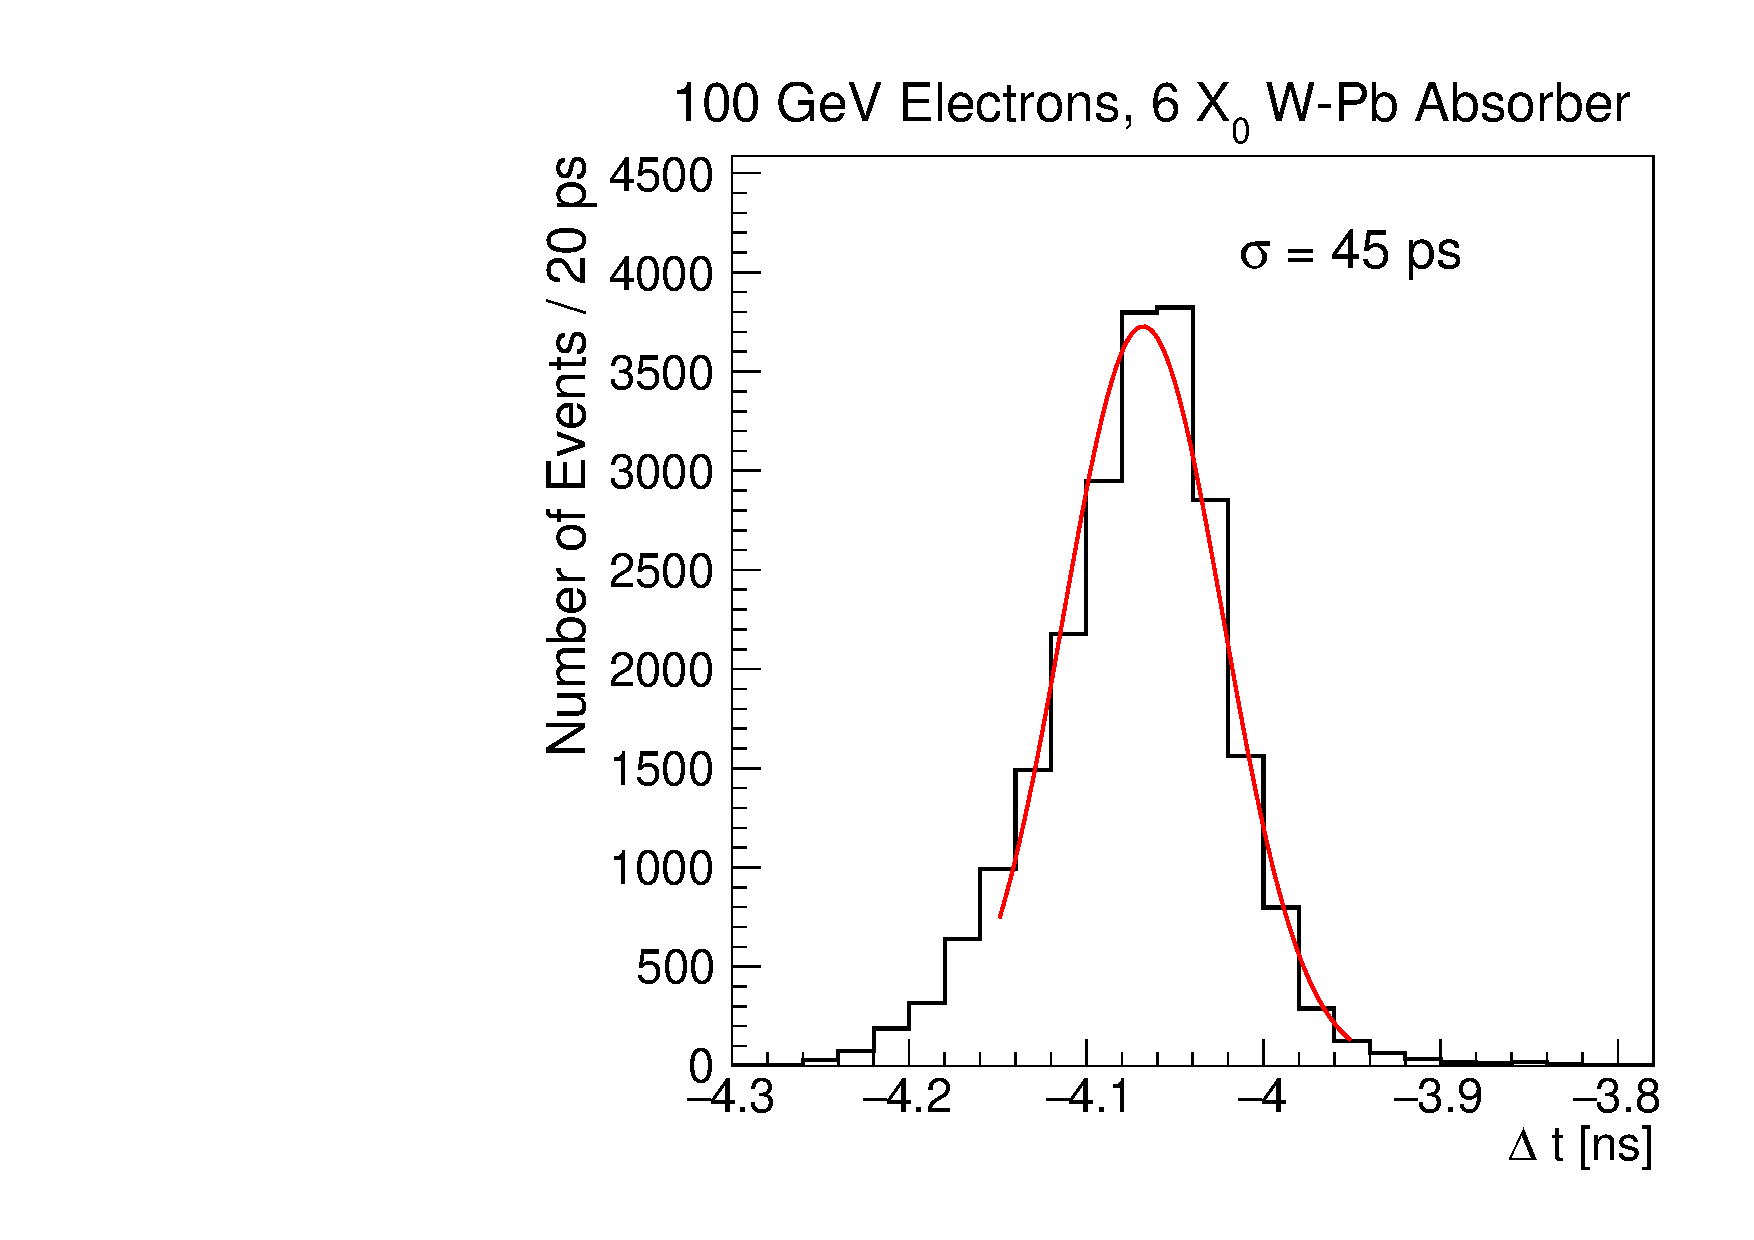
\includegraphics[width=0.49\textwidth]{figures/100GeV_deltaT.pdf} 
\caption{  } 
\label{fig:DeltaTVsAmplitude} 
\end{figure} 


We also study the dependence of the timestamp measurement as a function of the geometric
position of the incident beam particle as measured by the wire chambers in 
Figure~\ref{fig:DeltaTVsBeamXY}. A clear linear dependence is observed, and this 
geometric position non-uniformity of the time response adds significantly to the 
time resolution ($XX$~ps). Performing a correction for this non-uniformity results
in a time resolution of $YY$~ps.

%Fig: DeltaT vs Beam Location
\begin{figure}[htbp] 
\centering
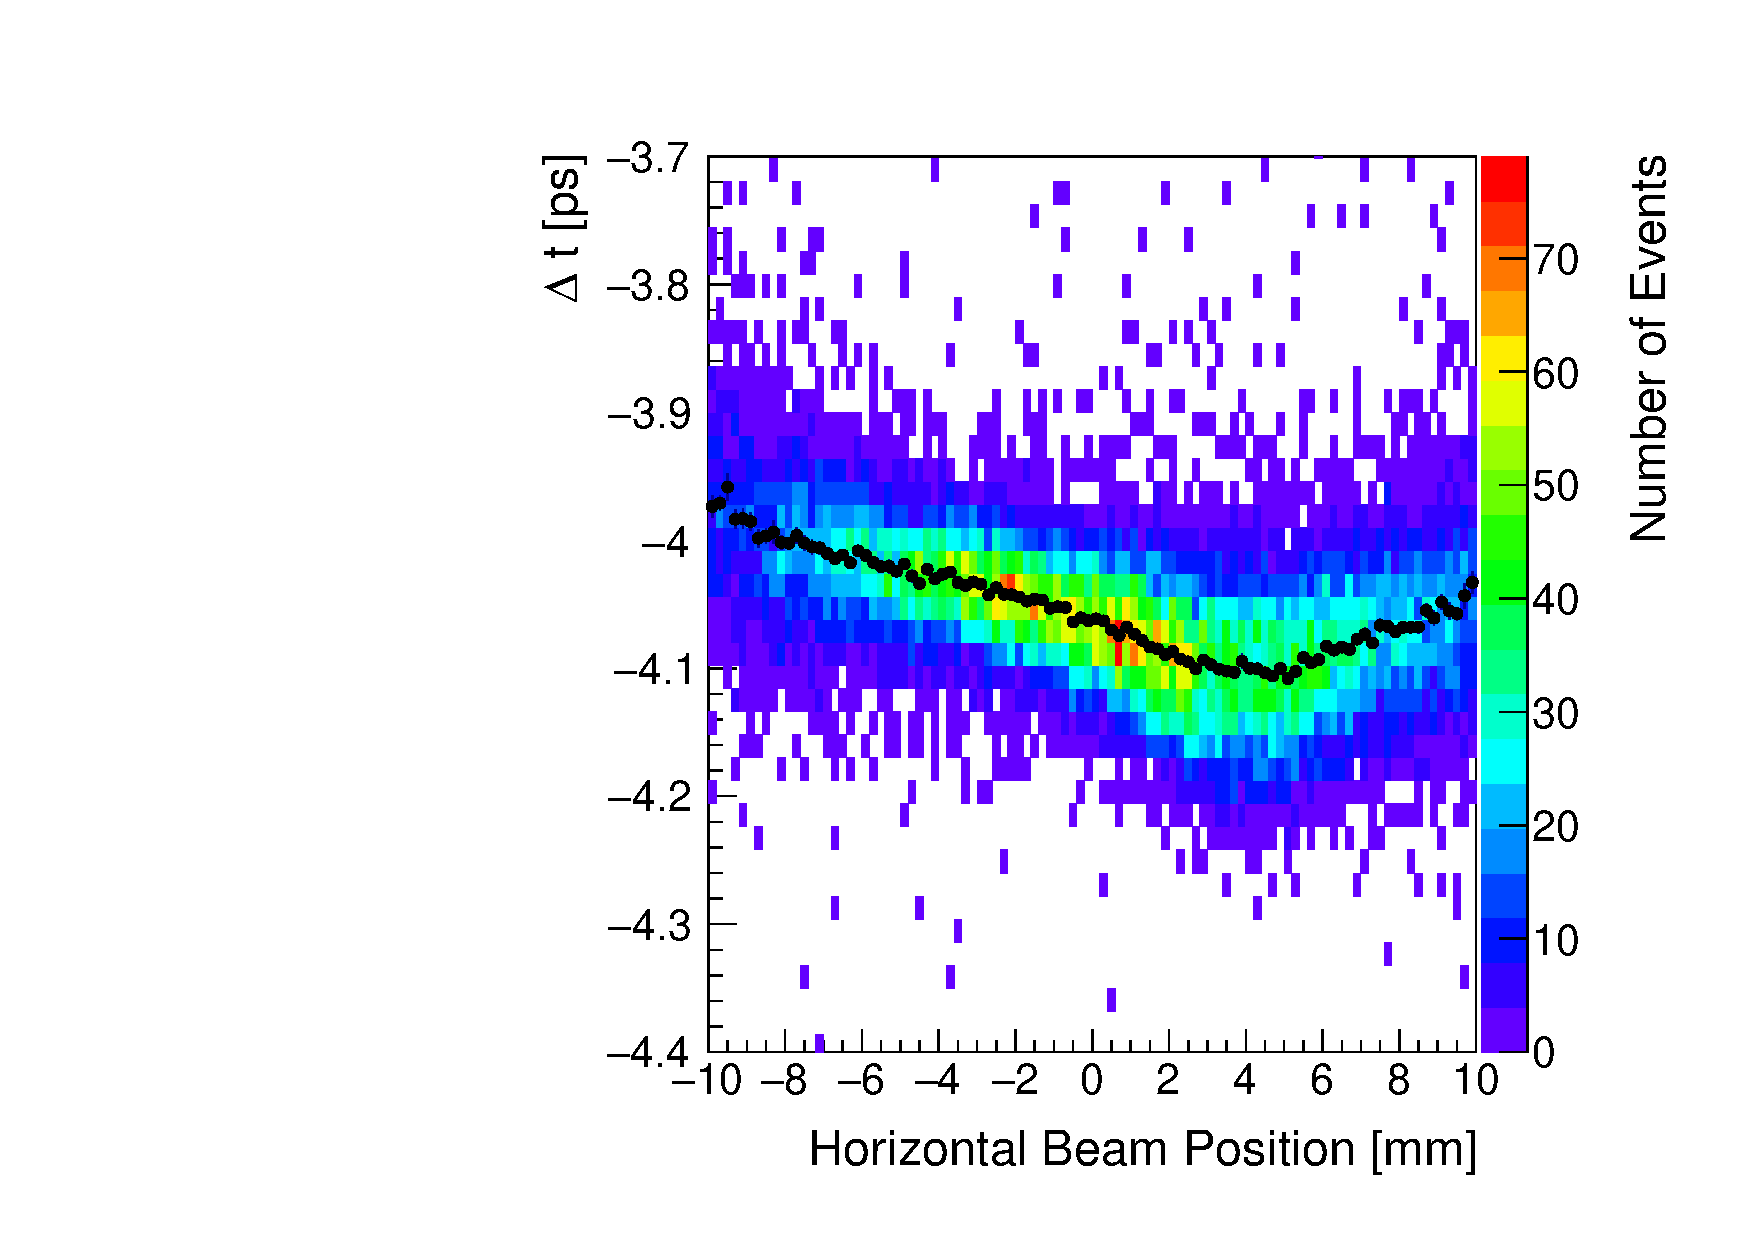
\includegraphics[width=0.49\textwidth]{figures/DeltaTVsHorizontalPosition.pdf} 
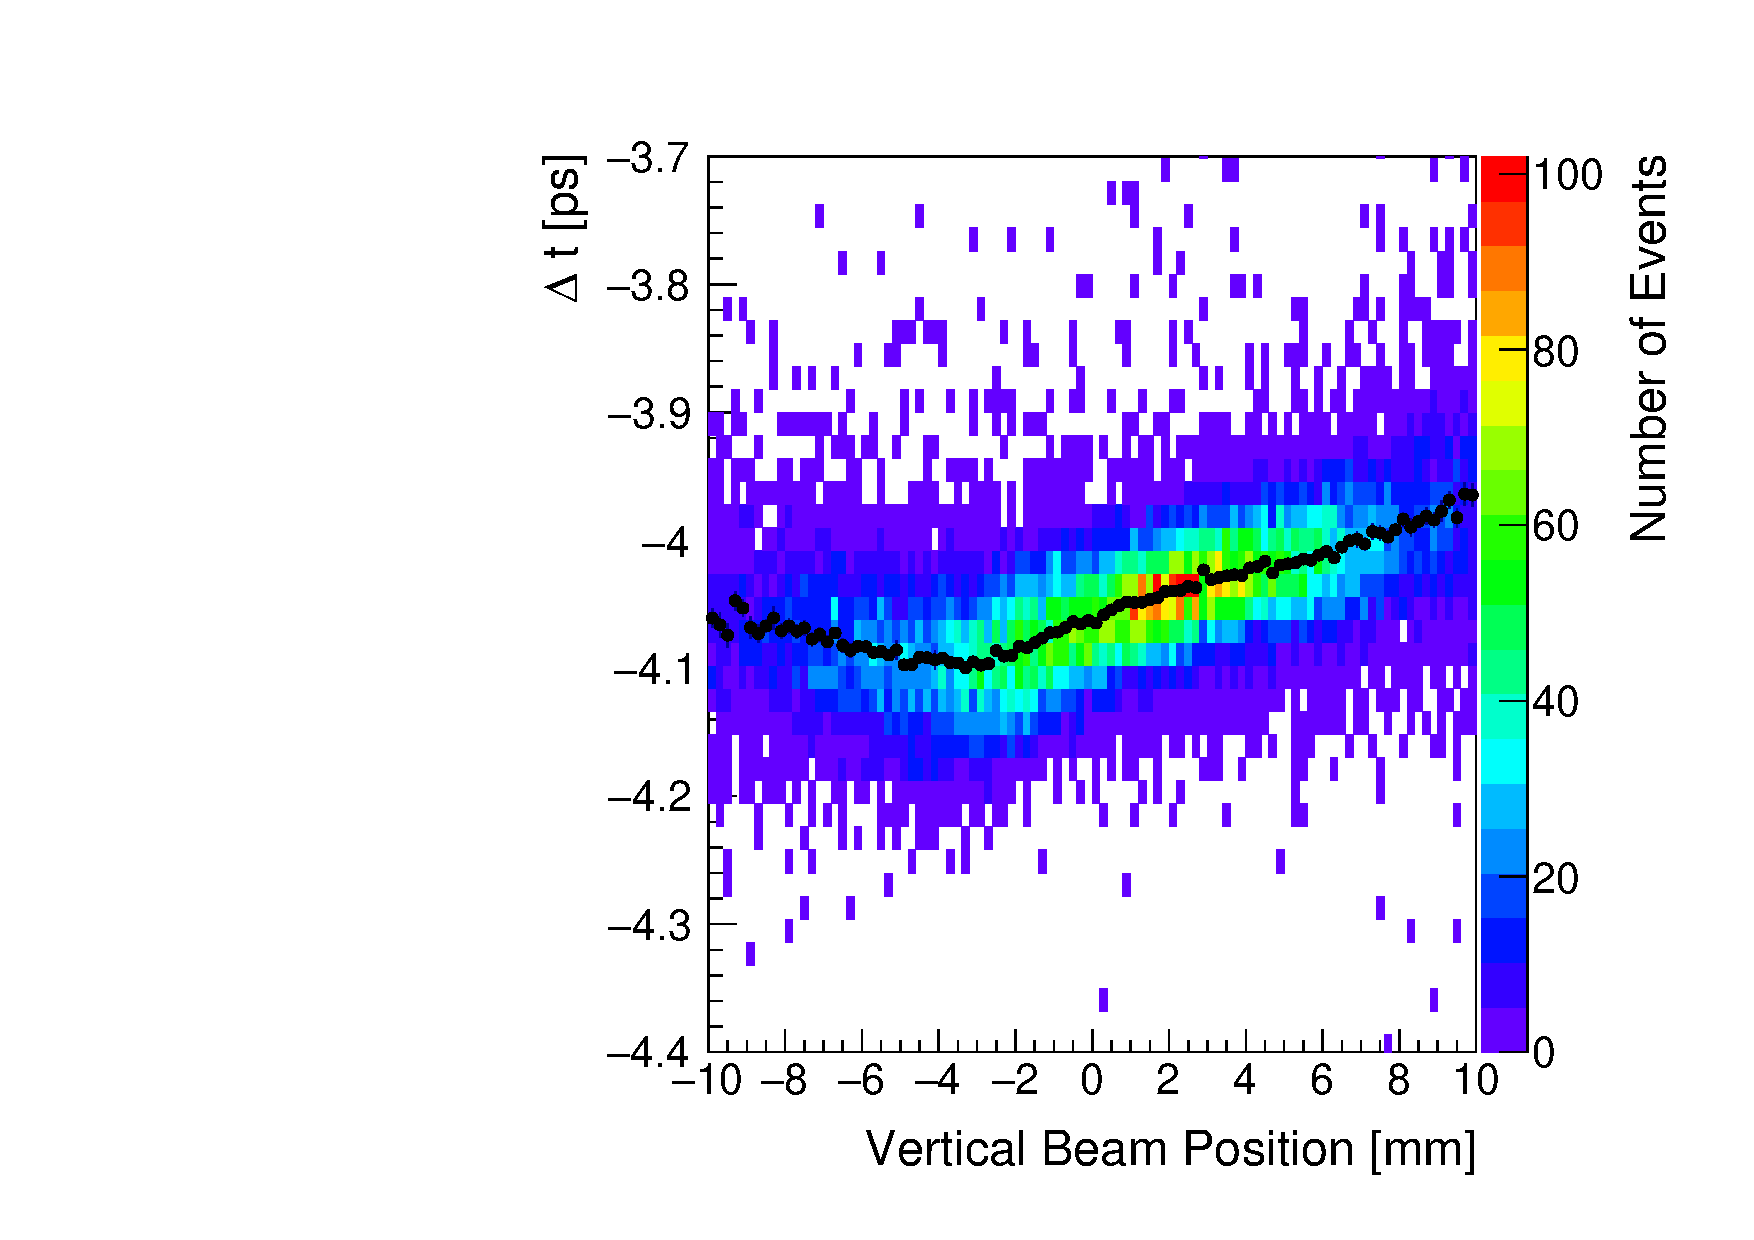
\includegraphics[width=0.49\textwidth]{figures/DeltaTVsVerticalPosition.pdf} 
\caption{ The distribution of the beam particle position measured by the wire chamber
and the time measured in the CdTe sensor relative to the Photek reference detector
is shown in the color scale. The mean value of the time measured in the CdTe sensor as a function
of the beam particle position is shown in the black points.} 
\label{fig:DeltaTVsBeamXY} 
\end{figure} 

An example of the distribution of the timestamp measurement after correcting for the
beam location for $100$~GeV electrons after $6$~$\mathrm{X}_{0}$ of absorber
material is shown in Figure~\ref{fig:DeltaT}. We extract the time measurement
resolution from this distribution as the width parameter of a gaussian fit.
The time measurement resolution has a mild dependence on the beam particle position
and is shown in Figure~\ref{fig:TimeResolutionVsBeamXY}.

The same measurement is performed on various beam energies and is summarized
in Figure~\ref{fig:ChargeVsEnergy}. Including the position non-uniformity 
correction, we obtain a time resolution of $25$~ps for electrons with energy above $100$~GeV. 

%Fig: example DeltaT plot
\begin{figure}[htbp] 
\centering
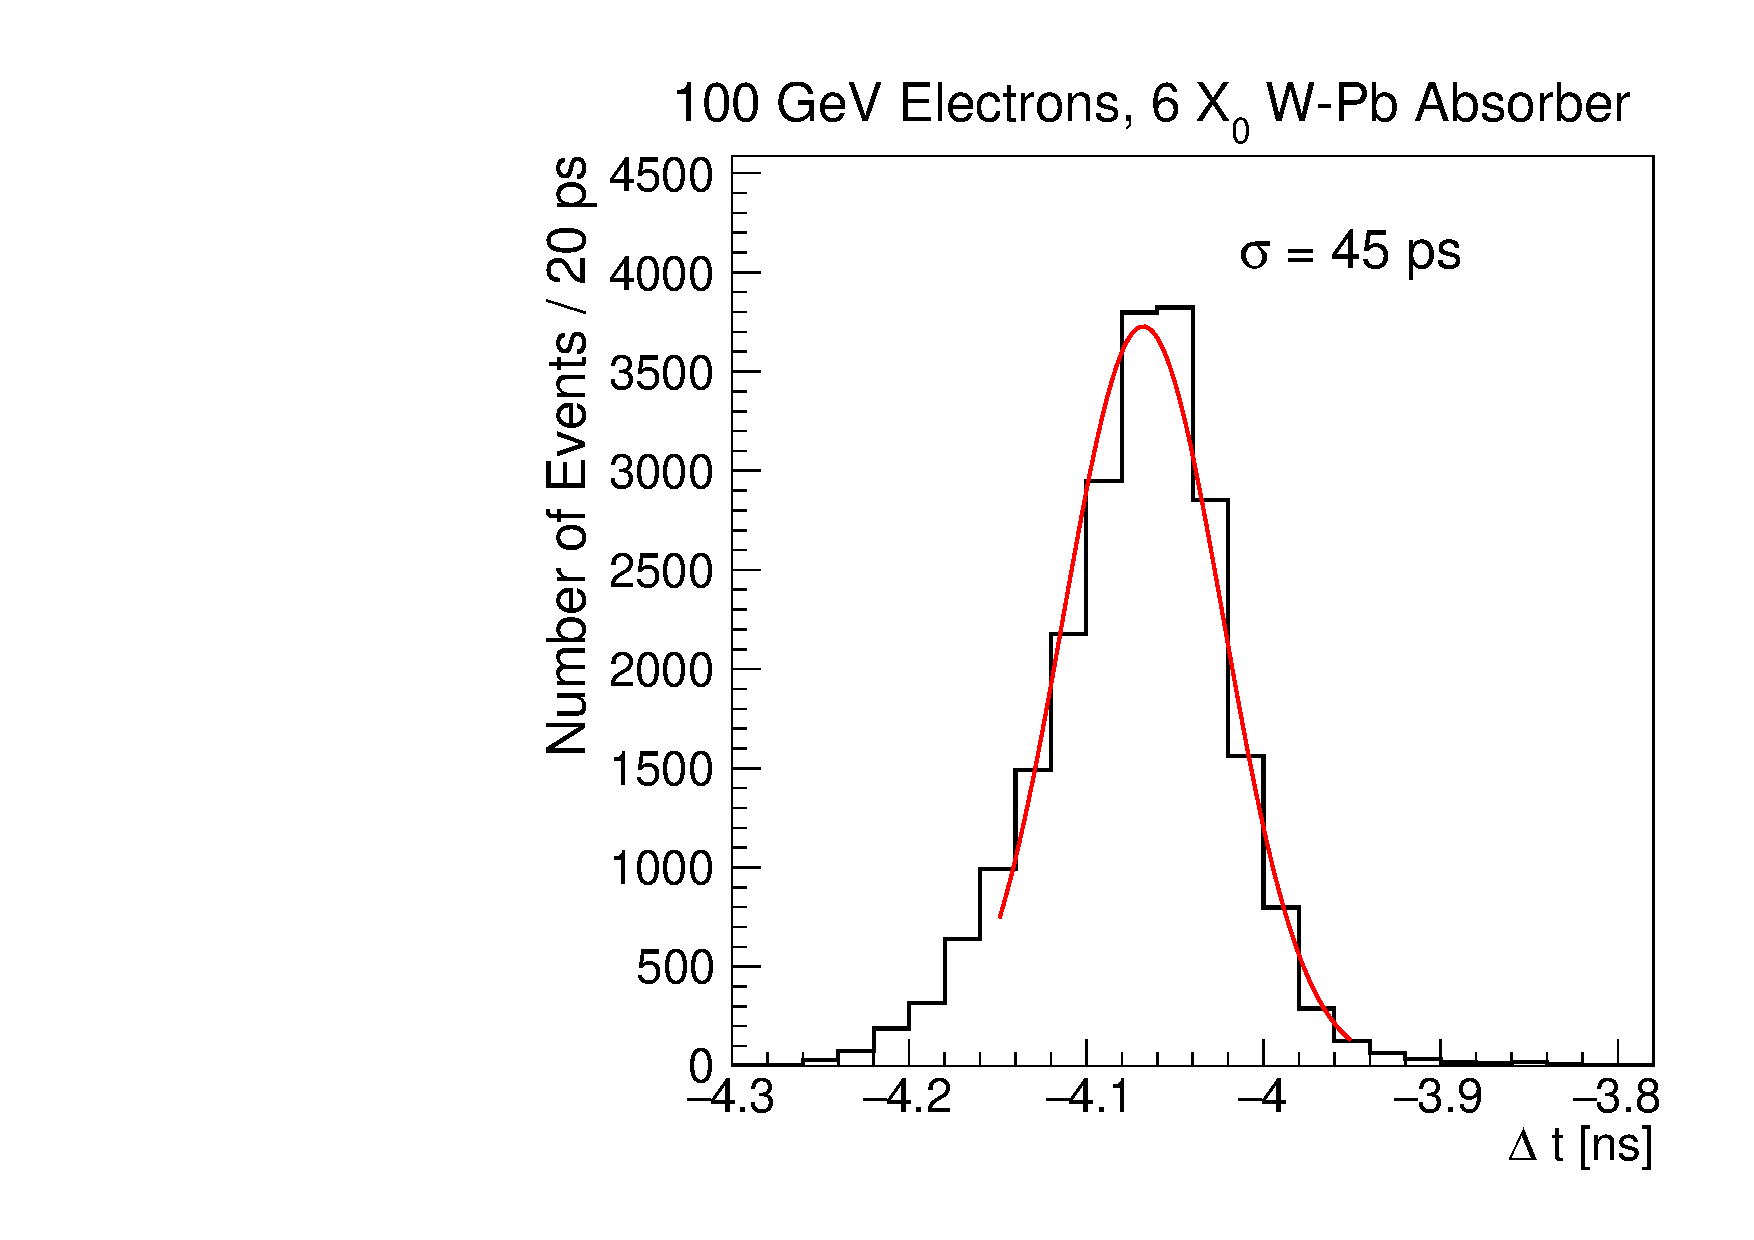
\includegraphics[width=0.49\textwidth]{figures/100GeV_deltaT.pdf} 
\caption{Distribution of the timestamp measurement in the CdTe sensor for a $100$~GeV
electron after $6$~$\mathrm{X}_{0}$ of tungsten absorber. } 
\label{fig:DeltaT} 
\end{figure} 


%Fig: Time Resolution vs Beam Location
\begin{figure}[htbp] 
\centering
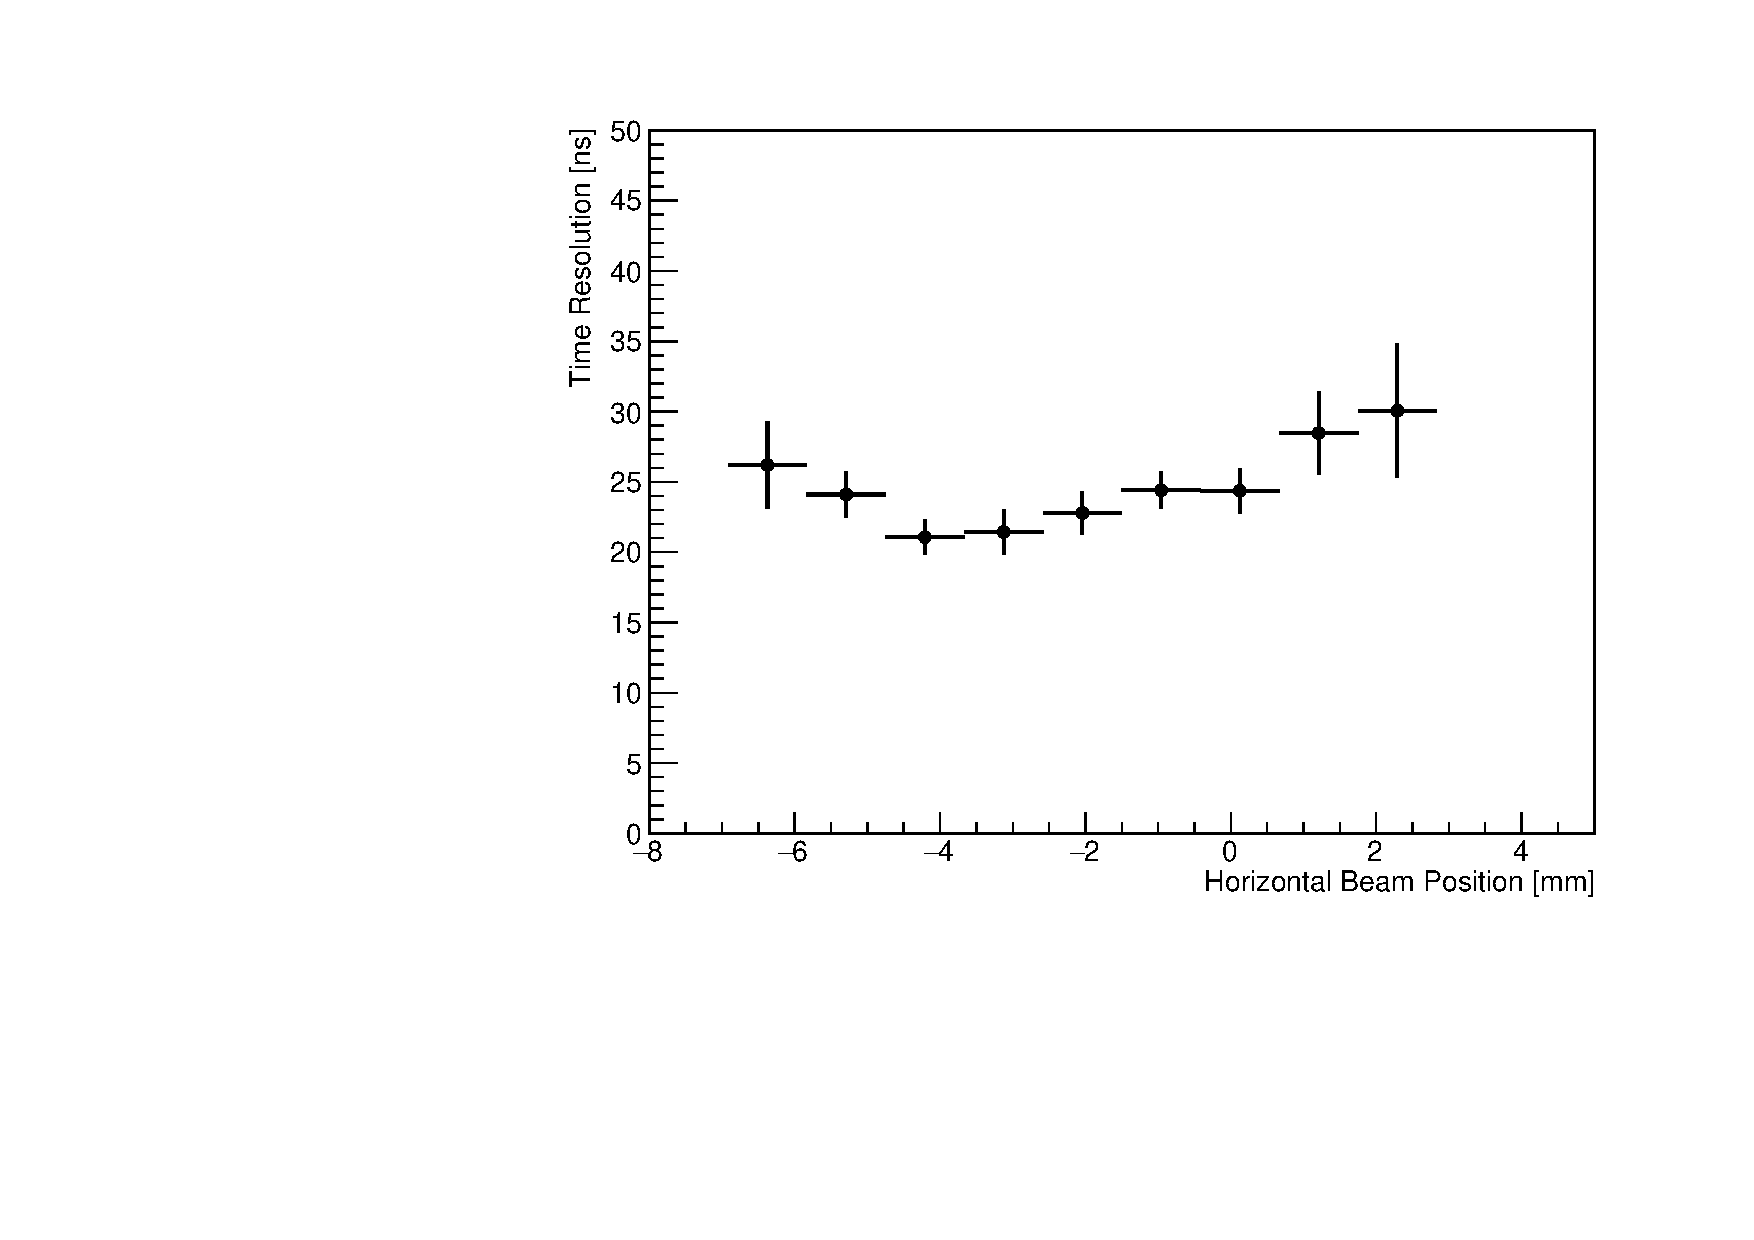
\includegraphics[width=0.49\textwidth]{figures/TimeResolutionVsBeamHorizontalPosition.pdf} 
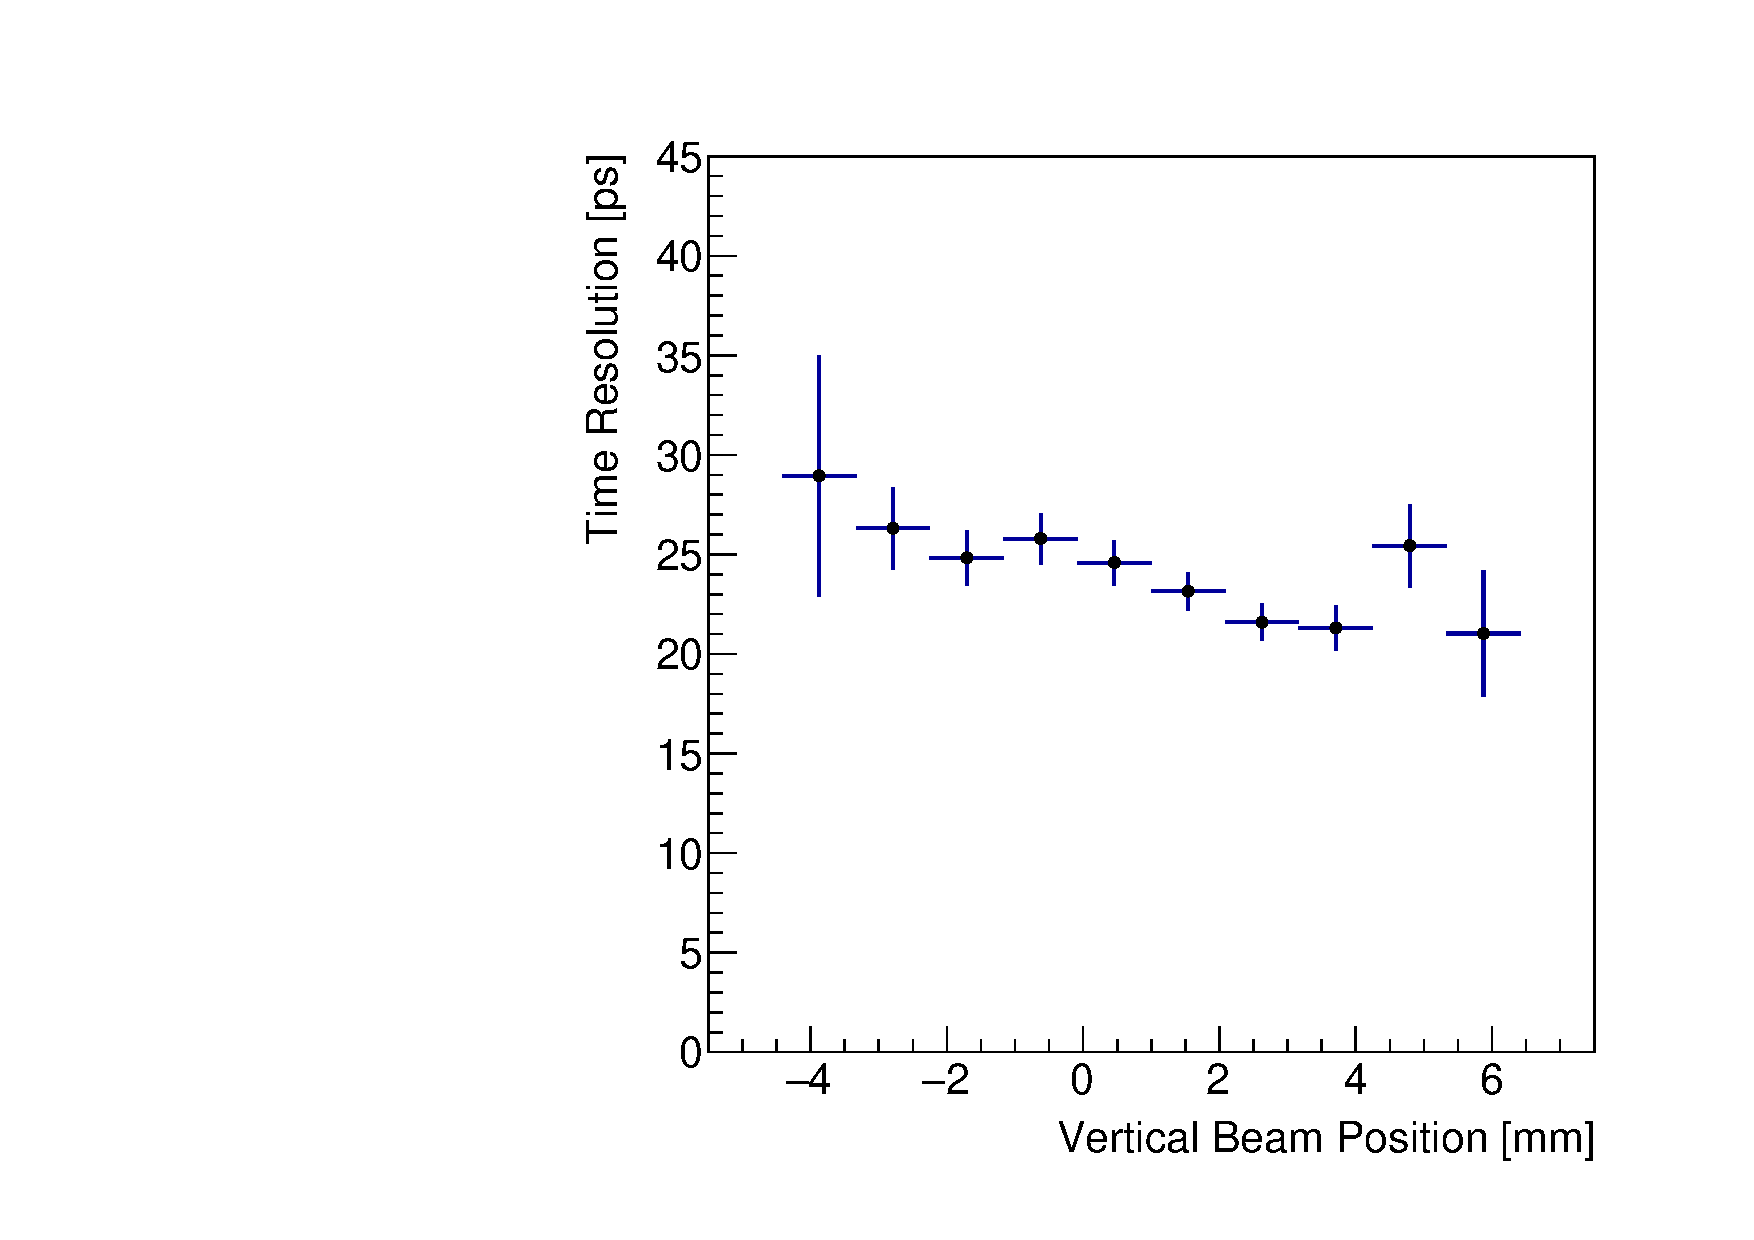
\includegraphics[width=0.49\textwidth]{figures/TimeResolutionVsBeamVerticalPosition.pdf} 
\caption{ The time resolution is measured as a function of the horizontal (left) and vertical (right)
beam position. }
\label{fig:TimeResolutionVsBeamXY} 
\end{figure} 




%Fig: Time resolution vs beam energy
\begin{figure}[htbp] 
\centering
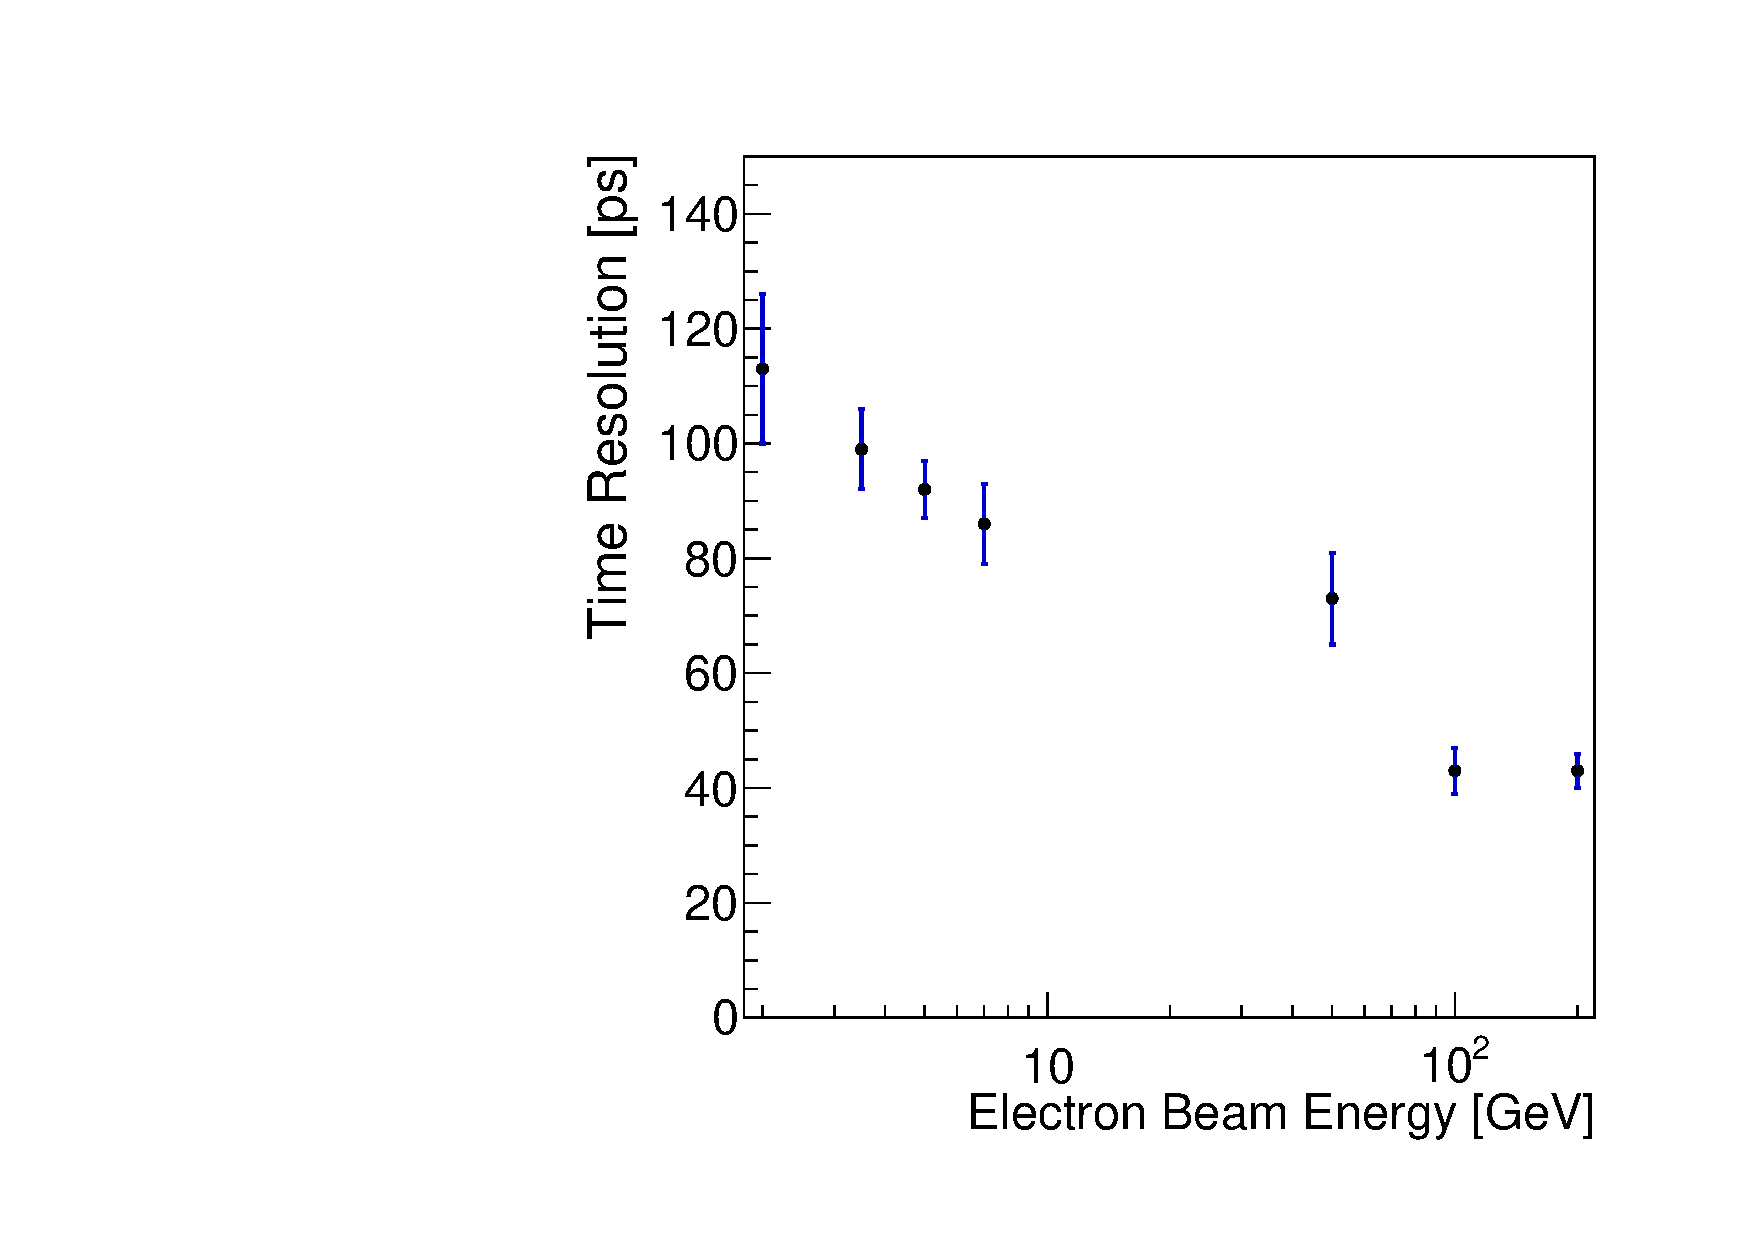
\includegraphics[width=0.49\textwidth]{figures/TimeResolutionVsEnergy.pdf} 
\caption{ The measured time resolution of the CdTe sensor is plotted as a function
of the electron beam energy. } 
\label{fig:ChargeVsEnergy} 
\end{figure} 



To further characterize the timing performance of the CdTe signals, we measure the
risetime, defined as the time for the signal to rise from $10\%$ to $90\%$ of the maximum
amplitude, for various electron beam energies. The distribution of risetime for
$100$~GeV electrons are shown on the left of Figure~\ref{fig:riseTime}. The 
measured risetime as a function of the beam energy is shown on the right of 
Figure~\ref{fig:riseTime}. We observe a risetime that is relatively stable
at around $1.3$~ns.


%Fig: riseTime vs energy
\begin{figure}[htbp] 
\centering
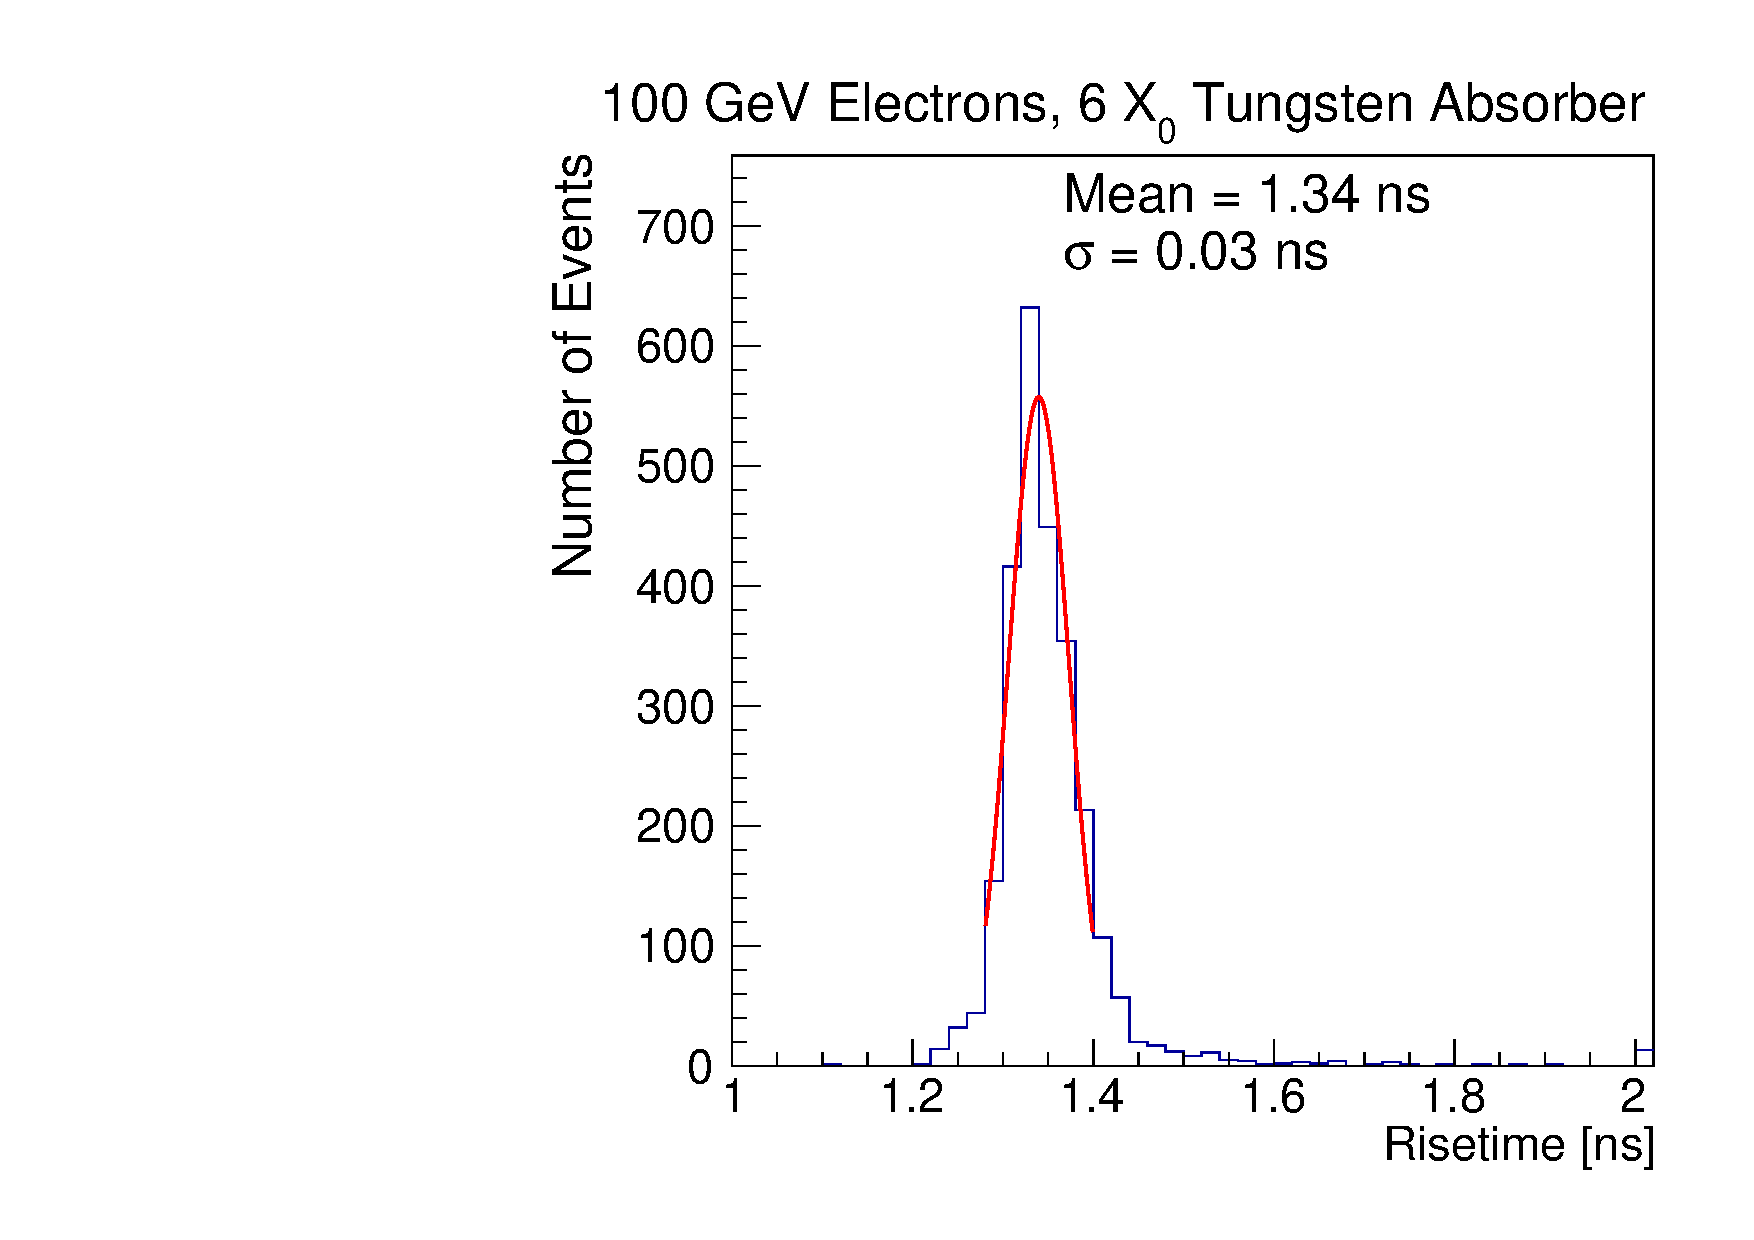
\includegraphics[width=0.49\textwidth]{figures/100GeV_risetime.pdf} 
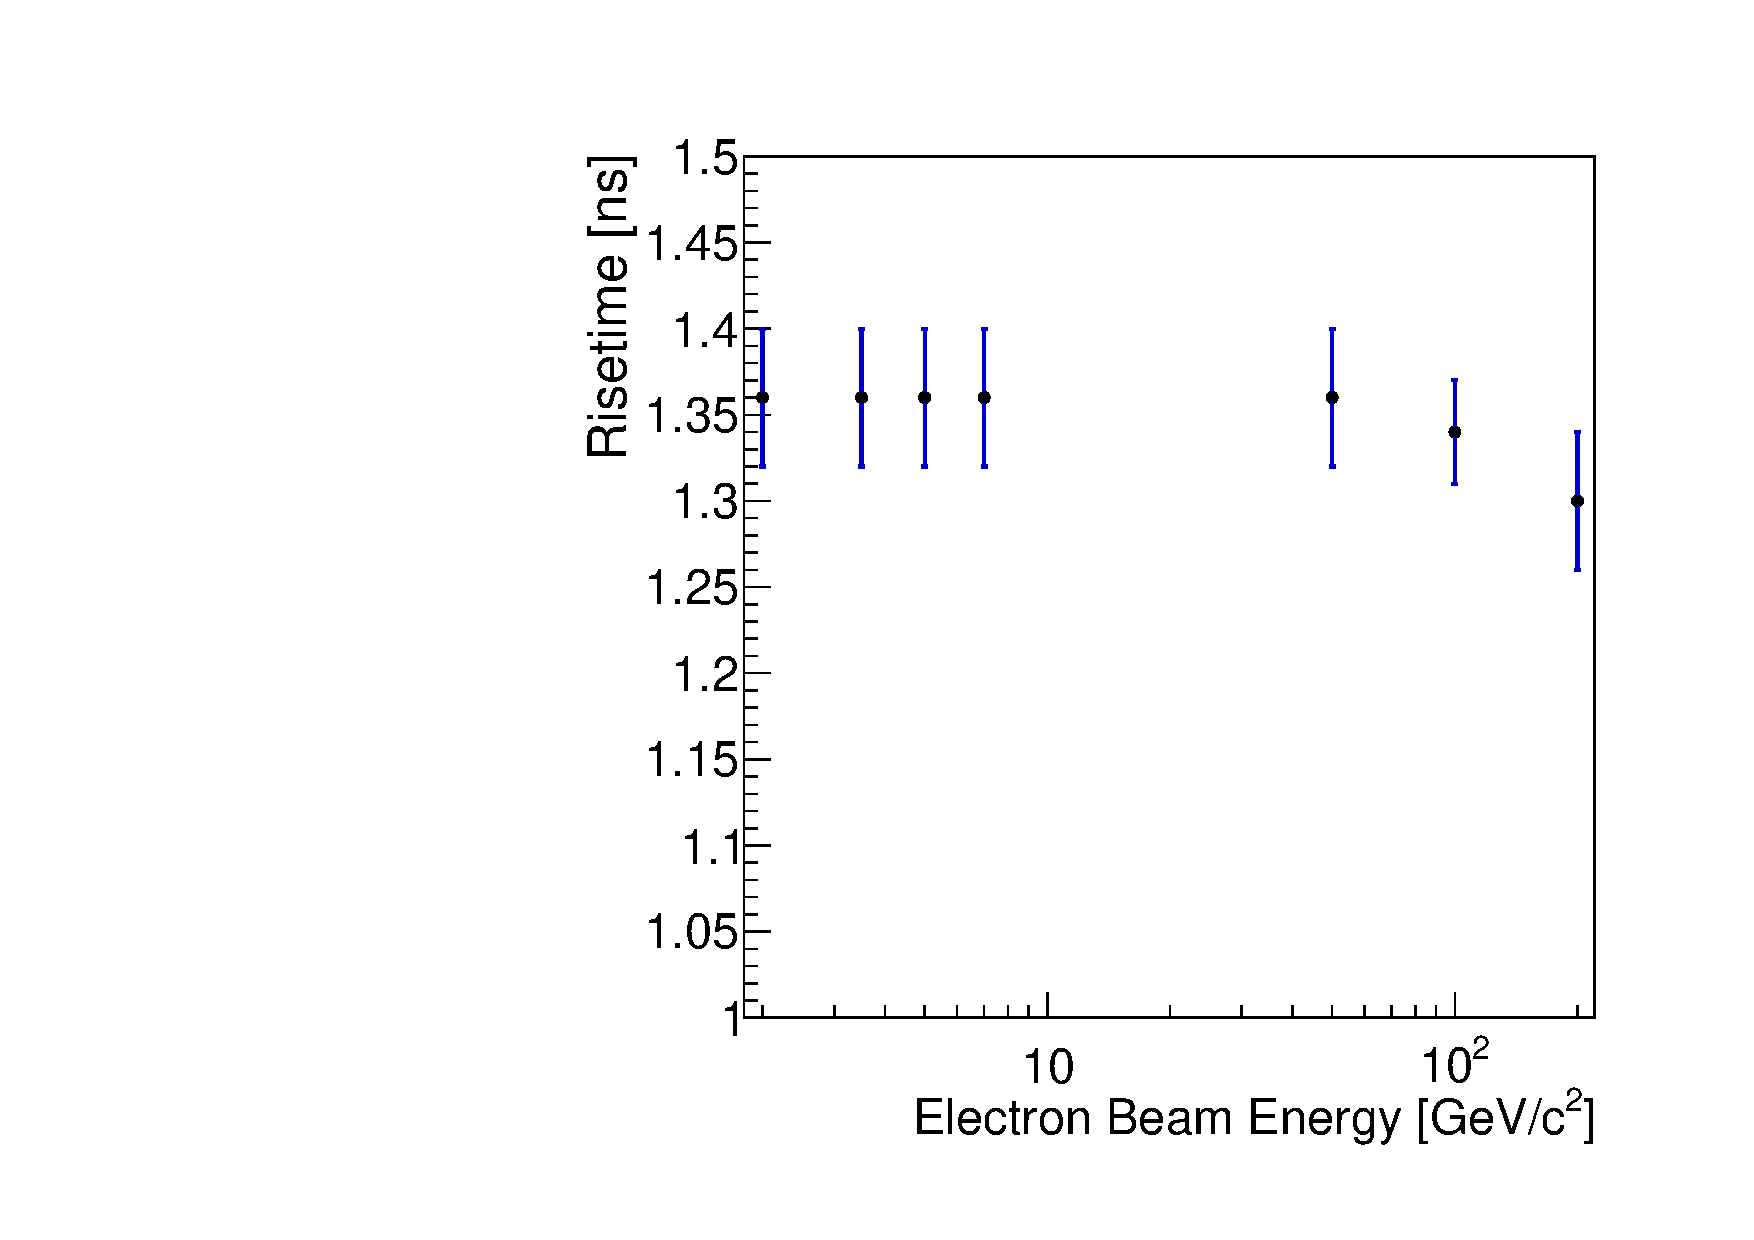
\includegraphics[width=0.49\textwidth]{figures/RisetimeVsEnergy.pdf} 
\caption{ Left: Distribution of risetime of the CdTe signal for $100$~GeV electrons. 
Right: Risetime of the CdTe signal is plotted as a function of the incident beam energy. } 
\label{fig:riseTime} 
\end{figure} 



%Extra studies
%MIP peak
%Charge vs beam location ( can we say anything about signal size on shower periphery? )
